% Options for packages loaded elsewhere
\PassOptionsToPackage{unicode}{hyperref}
\PassOptionsToPackage{hyphens}{url}
%
\documentclass[
]{article}
\usepackage{lmodern}
\usepackage{amssymb,amsmath}
\usepackage{ifxetex,ifluatex}
\ifnum 0\ifxetex 1\fi\ifluatex 1\fi=0 % if pdftex
  \usepackage[T1]{fontenc}
  \usepackage[utf8]{inputenc}
  \usepackage{textcomp} % provide euro and other symbols
\else % if luatex or xetex
  \usepackage{unicode-math}
  \defaultfontfeatures{Scale=MatchLowercase}
  \defaultfontfeatures[\rmfamily]{Ligatures=TeX,Scale=1}
\fi
% Use upquote if available, for straight quotes in verbatim environments
\IfFileExists{upquote.sty}{\usepackage{upquote}}{}
\IfFileExists{microtype.sty}{% use microtype if available
  \usepackage[]{microtype}
  \UseMicrotypeSet[protrusion]{basicmath} % disable protrusion for tt fonts
}{}
\makeatletter
\@ifundefined{KOMAClassName}{% if non-KOMA class
  \IfFileExists{parskip.sty}{%
    \usepackage{parskip}
  }{% else
    \setlength{\parindent}{0pt}
    \setlength{\parskip}{6pt plus 2pt minus 1pt}}
}{% if KOMA class
  \KOMAoptions{parskip=half}}
\makeatother
\usepackage{xcolor}
\IfFileExists{xurl.sty}{\usepackage{xurl}}{} % add URL line breaks if available
\IfFileExists{bookmark.sty}{\usepackage{bookmark}}{\usepackage{hyperref}}
\hypersetup{
  pdftitle={Assignment 1},
  pdfauthor={Stephen Giang},
  hidelinks,
  pdfcreator={LaTeX via pandoc}}
\urlstyle{same} % disable monospaced font for URLs
\usepackage[margin=1in]{geometry}
\usepackage{color}
\usepackage{fancyvrb}
\newcommand{\VerbBar}{|}
\newcommand{\VERB}{\Verb[commandchars=\\\{\}]}
\DefineVerbatimEnvironment{Highlighting}{Verbatim}{commandchars=\\\{\}}
% Add ',fontsize=\small' for more characters per line
\usepackage{framed}
\definecolor{shadecolor}{RGB}{248,248,248}
\newenvironment{Shaded}{\begin{snugshade}}{\end{snugshade}}
\newcommand{\AlertTok}[1]{\textcolor[rgb]{0.94,0.16,0.16}{#1}}
\newcommand{\AnnotationTok}[1]{\textcolor[rgb]{0.56,0.35,0.01}{\textbf{\textit{#1}}}}
\newcommand{\AttributeTok}[1]{\textcolor[rgb]{0.77,0.63,0.00}{#1}}
\newcommand{\BaseNTok}[1]{\textcolor[rgb]{0.00,0.00,0.81}{#1}}
\newcommand{\BuiltInTok}[1]{#1}
\newcommand{\CharTok}[1]{\textcolor[rgb]{0.31,0.60,0.02}{#1}}
\newcommand{\CommentTok}[1]{\textcolor[rgb]{0.56,0.35,0.01}{\textit{#1}}}
\newcommand{\CommentVarTok}[1]{\textcolor[rgb]{0.56,0.35,0.01}{\textbf{\textit{#1}}}}
\newcommand{\ConstantTok}[1]{\textcolor[rgb]{0.00,0.00,0.00}{#1}}
\newcommand{\ControlFlowTok}[1]{\textcolor[rgb]{0.13,0.29,0.53}{\textbf{#1}}}
\newcommand{\DataTypeTok}[1]{\textcolor[rgb]{0.13,0.29,0.53}{#1}}
\newcommand{\DecValTok}[1]{\textcolor[rgb]{0.00,0.00,0.81}{#1}}
\newcommand{\DocumentationTok}[1]{\textcolor[rgb]{0.56,0.35,0.01}{\textbf{\textit{#1}}}}
\newcommand{\ErrorTok}[1]{\textcolor[rgb]{0.64,0.00,0.00}{\textbf{#1}}}
\newcommand{\ExtensionTok}[1]{#1}
\newcommand{\FloatTok}[1]{\textcolor[rgb]{0.00,0.00,0.81}{#1}}
\newcommand{\FunctionTok}[1]{\textcolor[rgb]{0.00,0.00,0.00}{#1}}
\newcommand{\ImportTok}[1]{#1}
\newcommand{\InformationTok}[1]{\textcolor[rgb]{0.56,0.35,0.01}{\textbf{\textit{#1}}}}
\newcommand{\KeywordTok}[1]{\textcolor[rgb]{0.13,0.29,0.53}{\textbf{#1}}}
\newcommand{\NormalTok}[1]{#1}
\newcommand{\OperatorTok}[1]{\textcolor[rgb]{0.81,0.36,0.00}{\textbf{#1}}}
\newcommand{\OtherTok}[1]{\textcolor[rgb]{0.56,0.35,0.01}{#1}}
\newcommand{\PreprocessorTok}[1]{\textcolor[rgb]{0.56,0.35,0.01}{\textit{#1}}}
\newcommand{\RegionMarkerTok}[1]{#1}
\newcommand{\SpecialCharTok}[1]{\textcolor[rgb]{0.00,0.00,0.00}{#1}}
\newcommand{\SpecialStringTok}[1]{\textcolor[rgb]{0.31,0.60,0.02}{#1}}
\newcommand{\StringTok}[1]{\textcolor[rgb]{0.31,0.60,0.02}{#1}}
\newcommand{\VariableTok}[1]{\textcolor[rgb]{0.00,0.00,0.00}{#1}}
\newcommand{\VerbatimStringTok}[1]{\textcolor[rgb]{0.31,0.60,0.02}{#1}}
\newcommand{\WarningTok}[1]{\textcolor[rgb]{0.56,0.35,0.01}{\textbf{\textit{#1}}}}
\usepackage{graphicx,grffile}
\makeatletter
\def\maxwidth{\ifdim\Gin@nat@width>\linewidth\linewidth\else\Gin@nat@width\fi}
\def\maxheight{\ifdim\Gin@nat@height>\textheight\textheight\else\Gin@nat@height\fi}
\makeatother
% Scale images if necessary, so that they will not overflow the page
% margins by default, and it is still possible to overwrite the defaults
% using explicit options in \includegraphics[width, height, ...]{}
\setkeys{Gin}{width=\maxwidth,height=\maxheight,keepaspectratio}
% Set default figure placement to htbp
\makeatletter
\def\fps@figure{htbp}
\makeatother
\setlength{\emergencystretch}{3em} % prevent overfull lines
\providecommand{\tightlist}{%
  \setlength{\itemsep}{0pt}\setlength{\parskip}{0pt}}
\setcounter{secnumdepth}{-\maxdimen} % remove section numbering

\title{Assignment 1}
\author{Stephen Giang}
\date{}

\begin{document}
	\begin{center}
	\textbf{R Code} \\
	\textbf{Intro to Math Modeling} \\
	\textbf{Math 336} \\
	\textbf{Stephen Giang RedID: 823184070} \\ 
	\vspace{\baselineskip}
	\vspace{\baselineskip}
	\end{center}

\begin{Shaded}
\begin{Highlighting}[]
\CommentTok{# Problem 6, Exercise 2.1:}

\NormalTok{t <-}\StringTok{ }\KeywordTok{seq}\NormalTok{(}\DecValTok{2015}\NormalTok{,}\DecValTok{2018}\NormalTok{, }\DataTypeTok{length =} \DecValTok{100}\NormalTok{)}
\NormalTok{y1 <-}\StringTok{ }\ControlFlowTok{function}\NormalTok{(t) }\KeywordTok{sin}\NormalTok{(}\DecValTok{2}\OperatorTok{*}\NormalTok{pi}\OperatorTok{*}\NormalTok{(t }\OperatorTok{-}\StringTok{ }\FloatTok{.1}\NormalTok{))}
\NormalTok{y2 <-}\StringTok{ }\ControlFlowTok{function}\NormalTok{(t) (}\KeywordTok{cos}\NormalTok{(}\DecValTok{2}\OperatorTok{*}\NormalTok{pi}\OperatorTok{*}\NormalTok{t))}\OperatorTok{^}\DecValTok{2}

\KeywordTok{plot}\NormalTok{ (t,}\KeywordTok{y1}\NormalTok{(t), }\StringTok{'l'}\NormalTok{, }\DataTypeTok{col=}\StringTok{'blue'}\NormalTok{, }\DataTypeTok{ylab=}\StringTok{'Functions'}\NormalTok{, }\DataTypeTok{xlab =} \StringTok{'Time'}\NormalTok{, }
      \DataTypeTok{main =} \StringTok{'Functions over Time'}\NormalTok{ ,}\DataTypeTok{panel.first=}\KeywordTok{grid}\NormalTok{())}
\KeywordTok{lines}\NormalTok{(t,}\KeywordTok{y2}\NormalTok{(t), }\StringTok{'l'}\NormalTok{, }\DataTypeTok{col=}\StringTok{'red'}\NormalTok{)}

\NormalTok{text <-}\StringTok{ }\KeywordTok{c}\NormalTok{(}\KeywordTok{expression}\NormalTok{(y[}\DecValTok{1}\NormalTok{] }\OperatorTok{==}\StringTok{ }\KeywordTok{sin}\NormalTok{(}\DecValTok{2} \OperatorTok{*}\NormalTok{pi}\OperatorTok{*}\StringTok{ }\NormalTok{(t }\OperatorTok{-}\StringTok{ }\FloatTok{.1}\NormalTok{))),}\KeywordTok{expression}\NormalTok{(y[}\DecValTok{2}\NormalTok{] }\OperatorTok{==}\StringTok{ }\NormalTok{cos}\OperatorTok{^}\DecValTok{2}\OperatorTok{*}\NormalTok{(}\DecValTok{2}\OperatorTok{*}\NormalTok{pi}\OperatorTok{*}\NormalTok{t)))}
\KeywordTok{legend}\NormalTok{(}\StringTok{'topright'}\NormalTok{, }\DataTypeTok{legend=}\NormalTok{text , }\DataTypeTok{text.width =} \KeywordTok{strwidth}\NormalTok{(text)[}\DecValTok{1}\NormalTok{]}\OperatorTok{*}\FloatTok{1.2}\NormalTok{ , }
       \DataTypeTok{col=}\KeywordTok{c}\NormalTok{(}\StringTok{'blue'}\NormalTok{,}\StringTok{'red'}\NormalTok{) , }\DataTypeTok{lty=}\DecValTok{1}\NormalTok{ , }\DataTypeTok{cex=}\DecValTok{1}\NormalTok{ )}
\end{Highlighting}
\end{Shaded}

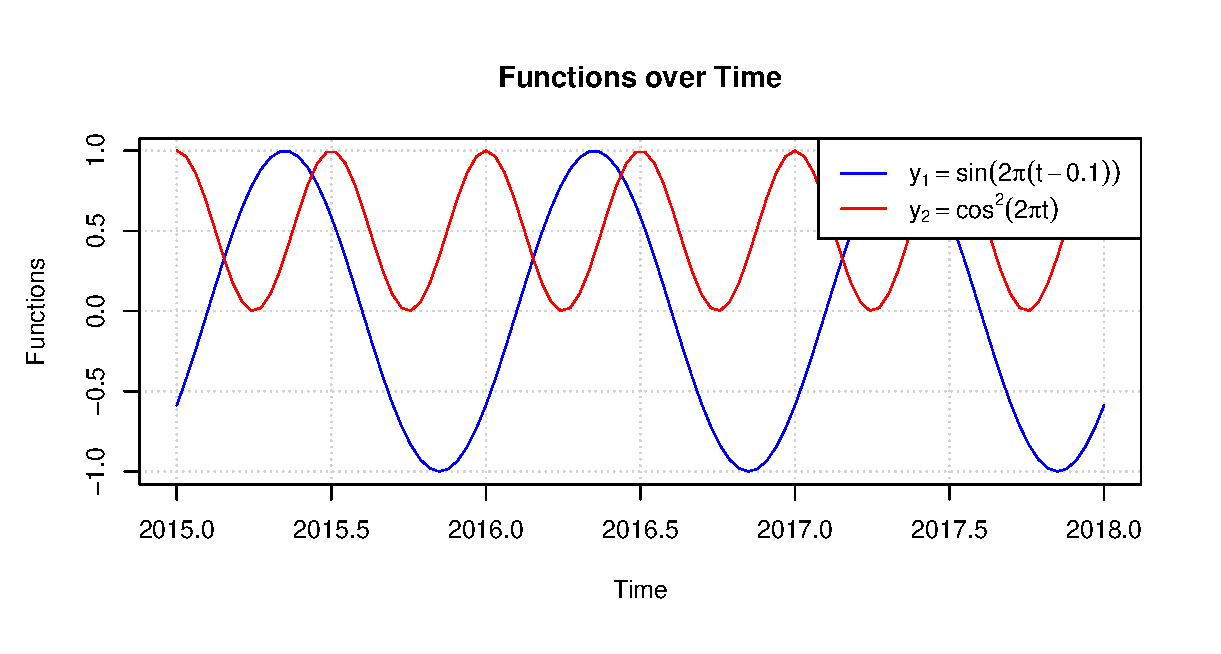
\includegraphics{Figures/prob6}
\newpage
\begin{Shaded}
\begin{Highlighting}[]
\CommentTok{# Problem 7, Exercise 2.4}

\NormalTok{A <-}\StringTok{ }\KeywordTok{matrix}\NormalTok{(}\KeywordTok{c}\NormalTok{(}\OperatorTok{-}\DecValTok{3}\NormalTok{, }\DecValTok{-2}\NormalTok{, }\DecValTok{2}\NormalTok{, }\DecValTok{2}\NormalTok{, }\DecValTok{-1}\NormalTok{, }\DecValTok{1}\NormalTok{, }\DecValTok{1}\NormalTok{ , }\DecValTok{1}\NormalTok{, }\DecValTok{-4}\NormalTok{),}\DataTypeTok{nrow=} \DecValTok{3}\NormalTok{)}
\NormalTok{b <-}\StringTok{ }\KeywordTok{matrix}\NormalTok{(}\KeywordTok{c}\NormalTok{(}\DecValTok{1}\NormalTok{, }\DecValTok{2}\NormalTok{, }\DecValTok{0}\NormalTok{))}
\NormalTok{x <-}\StringTok{ }\KeywordTok{solve}\NormalTok{(A,b)}

\NormalTok{printAnswer <-}\StringTok{ }\KeywordTok{c}\NormalTok{(}\KeywordTok{paste}\NormalTok{(}\StringTok{'x ='}\NormalTok{,x[}\DecValTok{1}\NormalTok{]),}\KeywordTok{paste}\NormalTok{(}\StringTok{'y ='}\NormalTok{,x[}\DecValTok{2}\NormalTok{]),}\KeywordTok{paste}\NormalTok{(}\StringTok{'z ='}\NormalTok{,x[}\DecValTok{3}\NormalTok{]))}
\KeywordTok{matrix}\NormalTok{(printAnswer)}
\end{Highlighting}
\end{Shaded}

\begin{verbatim}
##      [,1]                    
## [1,] "x = -1"                
## [2,] "y = -0.666666666666667"
## [3,] "z = -0.666666666666667"
\end{verbatim}

\newpage
\begin{Shaded}
\begin{Highlighting}[]
\CommentTok{# Problem 8, Exercise 2.5}

\KeywordTok{setwd}\NormalTok{(}\StringTok{'C:/Users/Stephen Giang/Documents/Math336Files/data'}\NormalTok{)}
\NormalTok{readData <-}\StringTok{ }\KeywordTok{read.csv}\NormalTok{(}\StringTok{'CA042239T.csv'}\NormalTok{)}

\NormalTok{readData <-}\StringTok{ }\NormalTok{readData[}\DecValTok{85}\OperatorTok{:}\KeywordTok{dim}\NormalTok{(readData)[}\DecValTok{1}\NormalTok{],]}
\NormalTok{readData}\OperatorTok{$}\NormalTok{TMAX..F. <-}\StringTok{ }\KeywordTok{as.numeric}\NormalTok{(readData}\OperatorTok{$}\NormalTok{TMAX..F.)}
\NormalTok{readData}\OperatorTok{$}\NormalTok{TMEAN..F. <-}\StringTok{ }\KeywordTok{as.numeric}\NormalTok{(readData}\OperatorTok{$}\NormalTok{TMEAN..F.)}
\NormalTok{readData}\OperatorTok{$}\NormalTok{TMIN..F. <-}\StringTok{ }\KeywordTok{as.numeric}\NormalTok{(readData}\OperatorTok{$}\NormalTok{TMIN..F.)}


\NormalTok{organize <-}\StringTok{ }\ControlFlowTok{function}\NormalTok{(readData, yearStart, yearEnd, colNum) \{}
\NormalTok{  rowStart <-}\StringTok{ }\DecValTok{1} \OperatorTok{+}\StringTok{ }\DecValTok{12}\OperatorTok{*}\NormalTok{(yearStart }\OperatorTok{-}\StringTok{ }\NormalTok{readData}\OperatorTok{$}\NormalTok{YEAR[}\DecValTok{1}\NormalTok{])}
\NormalTok{  rowEnd <-}\StringTok{ }\DecValTok{1} \OperatorTok{+}\StringTok{ }\DecValTok{12}\OperatorTok{*}\NormalTok{(yearEnd }\OperatorTok{-}\StringTok{ }\NormalTok{readData}\OperatorTok{$}\NormalTok{YEAR[}\DecValTok{1}\NormalTok{]) }\OperatorTok{+}\StringTok{ }\DecValTok{11}
  
\NormalTok{  dataRow <-}\StringTok{ }\KeywordTok{matrix}\NormalTok{( }\KeywordTok{c}\NormalTok{(readData[rowStart}\OperatorTok{:}\NormalTok{(rowStart}\OperatorTok{+}\DecValTok{11}\NormalTok{),colNum]),}\DataTypeTok{nrow=}\DecValTok{1}\NormalTok{)}
\NormalTok{  dataMatrix <-}\StringTok{ }\NormalTok{dataRow}
  
\NormalTok{  rowSeq <-}\StringTok{ }\KeywordTok{seq}\NormalTok{((rowStart}\OperatorTok{+}\DecValTok{12}\NormalTok{), rowEnd, }\DataTypeTok{by=}\DecValTok{12}\NormalTok{)}
  \ControlFlowTok{for}\NormalTok{ (row }\ControlFlowTok{in}\NormalTok{ rowSeq) \{}
\NormalTok{    dataRow <-}\StringTok{ }\KeywordTok{matrix}\NormalTok{( }\KeywordTok{c}\NormalTok{(readData[row}\OperatorTok{:}\NormalTok{(row}\OperatorTok{+}\DecValTok{11}\NormalTok{),colNum]),}\DataTypeTok{nrow=}\DecValTok{1}\NormalTok{)}
\NormalTok{    dataMatrix <-}\StringTok{ }\KeywordTok{rbind}\NormalTok{(dataMatrix, dataRow)}
\NormalTok{  \}}
  
  \KeywordTok{colnames}\NormalTok{(dataMatrix) <-}\StringTok{ }\KeywordTok{c}\NormalTok{(}\StringTok{'Jan'}\NormalTok{,}\StringTok{'Feb'}\NormalTok{, }\StringTok{'Mar'}\NormalTok{,}
                           \StringTok{'Apr'}\NormalTok{, }\StringTok{'May'}\NormalTok{, }\StringTok{'Jun'}\NormalTok{,}
                           \StringTok{'Jul'}\NormalTok{, }\StringTok{'Aug'}\NormalTok{, }\StringTok{'Sep'}\NormalTok{,}
                           \StringTok{'Oct'}\NormalTok{, }\StringTok{'Nov'}\NormalTok{, }\StringTok{'Dec'}\NormalTok{)}
  
  
  \KeywordTok{return}\NormalTok{(dataMatrix)}
\NormalTok{\}}


\NormalTok{PartA <-}\StringTok{ }\KeywordTok{organize}\NormalTok{(readData, }\DecValTok{1961}\NormalTok{, }\DecValTok{1990}\NormalTok{, }\DecValTok{4}\NormalTok{) }\CommentTok{#TMAX}
\NormalTok{PartA}
\end{Highlighting}
\end{Shaded}
\newpage
\begin{verbatim}
##        Jan  Feb  Mar  Apr  May  Jun  Jul  Aug  Sep  Oct  Nov  Dec
##  [1,] 53.8 55.7 53.0 64.3 64.2 81.3 87.6 85.0 76.3 69.3 54.0 48.9
##  [2,] 48.2 47.0 46.7 68.3 63.6 74.9 83.8 88.1 82.5 70.6 64.3 54.9
##  [3,] 46.1 61.8 53.7 55.0 68.3 70.6 85.7 83.3 80.1 70.1 58.5 54.4
##  [4,] 48.7 52.2 49.7 55.6 62.3 74.9 86.8 85.3 80.4 75.3 51.9 50.8
##  [5,] 50.7 52.4 49.9 56.7 66.6 69.8 84.4 84.9 73.3 76.8 59.1 46.9
##  [6,] 46.9 46.2 58.7 66.5 72.5 78.4 84.7 86.6 80.5 69.6 58.9 50.2
##  [7,] 51.0 55.0 54.2 47.8 65.0 70.9 86.6 86.5 74.8 74.4 61.4 43.3
##  [8,] 47.6 57.0 55.7 59.5 67.6 76.0 83.8 78.9 78.9 69.4 58.6 47.0
##  [9,] 50.8 44.0 52.6 61.7 69.5 73.8 83.4 89.3 81.4 65.6 57.0 58.1
## [10,] 53.1 55.5 55.1 56.5 69.4 77.2 86.6 86.6 78.6 67.3 58.5 47.9
## [11,] 51.8 52.7 57.5 56.8 60.6 73.7 85.1 85.6 79.5 64.7 55.9 44.3
## [12,] 51.6 56.8 66.8 63.1 71.2 77.3 86.0 81.6 77.7 62.8 54.0 47.8
## [13,] 45.8 47.9 44.3 59.0 70.3 78.4 84.1 82.3 76.7 69.7 55.0 54.9
## [14,] 47.6 53.3 55.3 59.6 67.3 81.3 81.7 82.2 81.9 67.0 58.3 50.6
## [15,] 53.2 50.4 49.7 47.1 65.8 75.6 83.0 82.7 79.7 66.7 59.5 53.5
## [16,] 54.7 52.7 52.8 56.2 69.1 76.8 83.1 78.5 72.0 67.1 60.5 54.6
## [17,] 48.2 59.2 50.0 63.0 57.3 77.3 84.0 82.3 76.3 71.6 63.7 57.6
## [18,] 50.5 50.3 54.6 55.0 66.3 78.6 84.7 82.7 75.2 74.1 54.1 47.5
## [19,] 43.2 47.9 51.2 60.8 66.1 78.5 82.7 79.4 83.9 69.9 55.6 56.2
## [20,] 49.8 54.4 50.2 59.3 57.6 74.3 85.1 81.5 80.0 70.4 62.9 57.8
## [21,] 54.6 56.8 52.0 63.3 67.4 83.6 85.3 87.2 80.5 63.7 62.7 58.1
## [22,] 47.2 53.1 51.3 59.5 66.5 71.9 81.7 85.6 76.1 67.8 54.2 50.4
## [23,] 52.4 51.4 51.2 52.1 67.1 73.4 82.0 81.2 80.0 68.4 56.5 52.6
## [24,] 53.8 58.4 60.5 60.0 76.2 76.3 82.3 81.2 79.3 63.3 55.2 45.4
## [25,] 47.7 51.7 53.5 66.2 68.2 79.5 84.7 84.1 70.7 67.4 55.0 53.5
## [26,] 58.7 53.5 59.2 61.5 68.2 78.2 79.5 86.6 71.4 65.3 62.8 55.5
## [27,] 52.6 53.1 50.5 68.1 67.8 79.7 80.0 81.5 79.8 70.8 57.3 47.5
## [28,] 52.0 58.6 62.1 60.6 69.0 78.2 86.1 83.0 79.5 77.5 58.5 50.8
## [29,] 47.0 50.1 62.6 69.9 66.8 77.3 87.4 80.9 80.5 68.8 64.4 54.7
## [30,] 51.3 48.8 57.5 62.0 63.2 77.5 83.5 81.9 79.6 73.7 58.9 47.9
\end{verbatim}
\newpage
\begin{Shaded}
\begin{Highlighting}[]
\NormalTok{PartB <-}\StringTok{ }\KeywordTok{organize}\NormalTok{(readData, }\DecValTok{1961}\NormalTok{, }\DecValTok{1990}\NormalTok{, }\DecValTok{6}\NormalTok{) }\CommentTok{#TMIN}
\NormalTok{PartB}
\end{Highlighting}
\end{Shaded}

\begin{verbatim}
##        Jan  Feb  Mar  Apr  May  Jun  Jul  Aug  Sep  Oct  Nov  Dec
##  [1,] 26.7 28.8 31.7 35.0 37.4 52.4 54.6 53.2 41.4 36.7 28.7 27.3
##  [2,] 27.1 30.4 27.1 39.0 38.3 44.3 50.1 53.5 45.8 35.6 28.5 25.5
##  [3,] 24.9 33.7 28.4 29.4 39.8 44.2 53.2 52.8 46.7 40.1 32.5 24.8
##  [4,] 25.8 24.4 25.3 31.0 37.3 43.1 52.4 52.4 43.1 42.9 27.8 32.0
##  [5,] 30.0 28.4 28.6 33.3 37.8 39.6 50.8 52.1 40.4 38.6 33.3 29.0
##  [6,] 25.4 25.9 31.6 37.0 39.9 45.2 52.0 53.8 45.9 37.5 32.6 31.7
##  [7,] 30.2 29.9 32.9 28.2 39.4 42.2 54.3 55.1 48.7 36.1 32.6 23.3
##  [8,] 27.1 34.8 31.3 31.9 38.6 47.6 54.2 49.8 45.7 37.4 31.4 23.4
##  [9,] 31.6 28.4 29.2 38.0 37.0 44.5 52.7 55.0 49.5 35.1 36.2 26.6
## [10,] 28.6 28.2 30.0 28.5 39.6 45.8 55.5 56.4 45.0 37.1 30.9 26.1
## [11,] 25.4 28.4 31.3 30.0 35.8 44.1 54.3 53.7 45.5 33.4 28.7 24.3
## [12,] 24.2 30.1 33.2 34.6 37.7 45.8 56.4 51.9 44.5 38.5 28.7 26.6
## [13,] 24.9 28.0 26.7 31.6 40.5 49.2 51.7 51.4 43.2 34.6 31.4 30.7
## [14,] 27.2 27.4 31.4 32.8 38.9 50.4 55.5 50.9 49.6 39.0 32.4 26.0
## [15,] 27.9 27.1 28.1 29.0 38.8 46.4 54.1 51.8 48.7 34.8 30.8 28.0
## [16,] 27.0 30.5 28.7 30.0 41.0 47.8 52.2 47.7 47.8 39.8 34.8 25.1
## [17,] 29.6 27.8 26.0 34.0 35.0 49.4 53.1 55.0 47.9 39.5 33.5 33.8
## [18,] 31.6 32.6 35.7 33.7 40.9 51.9 54.7 53.0 45.8 42.0 30.3 24.9
## [19,] 26.6 24.2 31.0 35.4 39.5 50.9 53.1 50.8 50.2 40.0 31.5 29.6
## [20,] 34.6 34.8 31.5 35.5 36.8 47.9 56.6 52.0 47.6 42.5 34.6 33.2
## [21,] 31.6 30.7 31.7 36.2 40.9 52.3 55.7 55.9 49.9 36.2 34.3 31.7
## [22,] 28.3 31.2 31.9 34.9 39.8 43.9 52.7 55.2 46.0 35.0 31.6 28.4
## [23,] 30.6 31.8 34.5 32.5 41.0 45.2 52.3 54.4 53.3 43.1 35.8 33.9
## [24,] 32.9 29.0 34.8 34.8 45.1 46.9 56.6 54.7 50.4 36.4 30.7 29.0
## [25,] 29.6 29.0 29.3 39.7 40.2 48.3 55.7 52.5 42.7 37.9 31.5 30.7
## [26,] 33.4 31.2 35.4 36.4 41.9 49.4 51.7 56.3 42.8 36.8 33.7 28.6
## [27,] 26.7 28.5 30.9 37.7 41.0 47.9 49.7 51.1 46.1 43.0 32.6 25.2
## [28,] 28.5 31.0 31.4 34.7 39.1 46.7 54.6 53.3 44.8 41.2 32.4 28.5
## [29,] 26.6 28.6 35.9 39.6 40.1 46.9 55.1 51.1 45.5 38.5 34.7 28.9
## [30,] 28.0 25.7 32.2 38.2 40.4 48.6 55.9 52.0 48.9 38.7 32.8 24.7
\end{verbatim}
\newpage
\begin{Shaded}
\begin{Highlighting}[]
\NormalTok{PartC <-}\StringTok{ }\KeywordTok{organize}\NormalTok{(readData, }\DecValTok{1961}\NormalTok{, }\DecValTok{1990}\NormalTok{, }\DecValTok{5}\NormalTok{) }\CommentTok{#TMEAN}
\NormalTok{PartC}
\end{Highlighting}
\end{Shaded}

\begin{verbatim}
##        Jan  Feb  Mar  Apr  May  Jun  Jul  Aug  Sep  Oct  Nov  Dec
##  [1,] 40.2 42.2 42.4 49.7 50.8 66.8 71.1 69.1 58.9 53.0 41.4 38.1
##  [2,] 37.6 38.7 36.9 53.7 51.0 59.6 67.0 70.8 64.1 53.1 46.4 40.2
##  [3,] 35.5 47.8 41.0 42.2 54.1 57.4 69.5 68.1 63.4 55.1 45.5 39.6
##  [4,] 37.2 38.3 37.5 43.3 49.8 59.0 69.6 68.8 61.8 59.1 39.8 41.4
##  [5,] 40.4 40.4 39.2 45.0 52.2 54.7 67.6 68.5 56.9 57.7 46.2 38.0
##  [6,] 36.2 36.1 45.1 51.8 56.2 61.8 68.4 70.2 63.2 53.5 45.8 40.9
##  [7,] 40.6 42.4 43.6 38.0 52.2 56.6 70.5 70.8 61.7 55.3 47.0 33.3
##  [8,] 37.3 45.9 43.5 45.7 53.1 61.8 69.0 64.3 62.3 53.4 45.0 35.2
##  [9,] 41.2 36.2 40.9 49.8 53.3 59.2 68.1 72.2 65.5 50.4 46.6 42.3
## [10,] 40.9 41.9 42.5 42.5 54.5 61.5 71.1 71.5 61.8 52.2 44.7 37.0
## [11,] 38.6 40.6 44.4 43.4 48.2 58.9 69.7 69.7 62.5 49.0 42.4 34.3
## [12,] 37.9 43.4 50.0 48.8 54.4 61.6 71.2 66.7 61.1 50.6 41.4 37.2
## [13,] 35.4 38.0 35.5 45.3 55.4 63.8 67.9 66.8 59.9 52.2 43.2 42.8
## [14,] 37.4 40.3 43.3 46.2 53.1 65.8 68.6 66.6 65.7 53.0 45.4 38.3
## [15,] 40.5 38.8 38.9 38.0 52.3 61.0 68.6 67.2 64.2 50.7 45.2 40.7
## [16,] 40.8 41.6 40.7 43.1 55.1 62.3 67.6 63.1 59.9 53.5 47.6 39.9
## [17,] 38.9 43.5 38.0 48.5 46.1 63.4 68.6 68.6 62.1 55.5 48.7 45.7
## [18,] 41.0 41.5 45.2 44.4 53.6 65.3 69.7 67.9 60.5 58.0 42.2 36.2
## [19,] 34.9 36.0 41.1 48.1 52.8 64.7 67.9 65.1 67.0 54.9 43.5 42.9
## [20,] 42.2 44.6 40.8 47.4 47.2 61.1 70.8 66.8 63.8 56.5 48.7 45.5
## [21,] 43.1 43.7 41.9 49.8 54.1 67.9 70.5 71.5 65.2 49.9 48.5 44.9
## [22,] 37.8 42.2 41.6 47.2 53.2 57.9 67.2 70.4 61.1 51.4 42.9 39.4
## [23,] 41.5 41.6 42.9 42.3 54.0 59.3 67.2 67.8 66.6 55.8 46.2 43.2
## [24,] 43.3 43.7 47.7 47.4 60.7 61.6 69.4 68.0 64.9 49.9 42.9 37.2
## [25,] 38.6 40.4 41.4 53.0 54.2 64.0 70.2 68.3 56.7 52.6 43.3 42.1
## [26,] 46.1 42.3 47.3 49.0 55.0 63.8 65.6 71.4 57.1 51.0 48.2 42.1
## [27,] 39.7 40.8 40.7 52.9 54.4 63.8 64.9 66.3 63.0 56.9 44.9 36.4
## [28,] 40.2 44.8 46.8 47.7 54.1 62.4 70.4 68.1 62.2 59.3 45.5 39.7
## [29,] 36.8 39.4 49.2 54.7 53.4 62.1 71.3 66.0 63.0 53.7 49.5 41.8
## [30,] 39.7 37.3 44.9 50.1 51.8 63.1 69.7 67.0 64.3 56.2 45.9 36.3
\end{verbatim}
\newpage
\begin{Shaded}
\begin{Highlighting}[]
\CommentTok{#Problem 9, Exercise 2.7}

\KeywordTok{setwd}\NormalTok{(}\StringTok{'C:/Users/Stephen Giang/Documents/Math336Files/data'}\NormalTok{)}
\NormalTok{readData <-}\StringTok{ }\KeywordTok{read.csv}\NormalTok{(}\StringTok{'CA042239T.csv'}\NormalTok{)}

\NormalTok{readData <-}\StringTok{ }\NormalTok{readData[}\DecValTok{85}\OperatorTok{:}\KeywordTok{dim}\NormalTok{(readData)[}\DecValTok{1}\NormalTok{],]}
\NormalTok{readData}\OperatorTok{$}\NormalTok{TMAX..F. <-}\StringTok{ }\KeywordTok{as.numeric}\NormalTok{(readData}\OperatorTok{$}\NormalTok{TMAX..F.)}
\NormalTok{readData}\OperatorTok{$}\NormalTok{TMEAN..F. <-}\StringTok{ }\KeywordTok{as.numeric}\NormalTok{(readData}\OperatorTok{$}\NormalTok{TMEAN..F.)}
\NormalTok{readData}\OperatorTok{$}\NormalTok{TMIN..F. <-}\StringTok{ }\KeywordTok{as.numeric}\NormalTok{(readData}\OperatorTok{$}\NormalTok{TMIN..F.)}


\NormalTok{TMinMatrix <-}\StringTok{ }\ControlFlowTok{function}\NormalTok{(readData, yearStart, yearEnd) \{}
\NormalTok{  rowStart <-}\StringTok{ }\DecValTok{1} \OperatorTok{+}\StringTok{ }\DecValTok{12}\OperatorTok{*}\NormalTok{(yearStart }\OperatorTok{-}\StringTok{ }\NormalTok{readData}\OperatorTok{$}\NormalTok{YEAR[}\DecValTok{1}\NormalTok{])}
\NormalTok{  rowEnd <-}\StringTok{ }\DecValTok{1} \OperatorTok{+}\StringTok{ }\DecValTok{12}\OperatorTok{*}\NormalTok{(yearEnd }\OperatorTok{-}\StringTok{ }\NormalTok{readData}\OperatorTok{$}\NormalTok{YEAR[}\DecValTok{1}\NormalTok{]) }\OperatorTok{+}\StringTok{ }\DecValTok{11}
  
\NormalTok{  yearCol <-}\StringTok{ }\KeywordTok{matrix}\NormalTok{( }\KeywordTok{c}\NormalTok{( readData[rowStart}\OperatorTok{:}\NormalTok{rowEnd, }\DecValTok{2}\NormalTok{] }\OperatorTok{+}\StringTok{ }
\StringTok{                          }\NormalTok{((readData[rowStart}\OperatorTok{:}\NormalTok{rowEnd, }\DecValTok{3}\NormalTok{] }\OperatorTok{-}\StringTok{ }\DecValTok{1}\NormalTok{) }\OperatorTok{/}\StringTok{ }\DecValTok{12}\NormalTok{) ), }\DataTypeTok{ncol=}\DecValTok{1}\NormalTok{ )}
\NormalTok{  TMinCol <-}\StringTok{ }\KeywordTok{matrix}\NormalTok{( }\KeywordTok{c}\NormalTok{( readData[rowStart}\OperatorTok{:}\NormalTok{rowEnd, }\DecValTok{6}\NormalTok{]), }\DataTypeTok{ncol=}\DecValTok{1}\NormalTok{ )}
  
\NormalTok{  dataMatrix <-}\StringTok{ }\NormalTok{yearCol}
\NormalTok{  dataMatrix <-}\StringTok{ }\KeywordTok{cbind}\NormalTok{(dataMatrix, TMinCol)}
  
  \KeywordTok{return}\NormalTok{(dataMatrix)}
\NormalTok{\}}

\NormalTok{slope <-}\StringTok{ }\KeywordTok{seq}\NormalTok{(}\DecValTok{0}\NormalTok{,}\DecValTok{0}\NormalTok{,}\DataTypeTok{len=}\DecValTok{4}\NormalTok{)}
\NormalTok{slopeCount <-}\StringTok{ }\DecValTok{1}
\NormalTok{colorList <-}\StringTok{ }\KeywordTok{c}\NormalTok{(}\StringTok{'black'}\NormalTok{, }\StringTok{'red'}\NormalTok{,}\StringTok{'blue'}\NormalTok{,}\StringTok{'green'}\NormalTok{,}\StringTok{'yellow'}\NormalTok{)}
\NormalTok{colorCount <-}\StringTok{ }\DecValTok{2}

\NormalTok{TMinVals <-}\StringTok{ }\KeywordTok{TMinMatrix}\NormalTok{(readData, }\DecValTok{1951}\NormalTok{, }\DecValTok{2010}\NormalTok{)}
\KeywordTok{plot}\NormalTok{(TMinVals[,}\DecValTok{1}\NormalTok{], TMinVals[,}\DecValTok{2}\NormalTok{], }\StringTok{'l'}\NormalTok{, }\DataTypeTok{xlab=}\StringTok{'Year'}\NormalTok{,}\DataTypeTok{ylab=}\StringTok{'Minimum Temperature'}\NormalTok{, }
     \DataTypeTok{main=}\StringTok{'Minimum Temperature per Year'}\NormalTok{, }\DataTypeTok{col=}\NormalTok{ colorList[}\DecValTok{1}\NormalTok{], }\DataTypeTok{ylim=}\KeywordTok{range}\NormalTok{(}\DecValTok{35}\NormalTok{,}\DecValTok{42}\NormalTok{))}


\NormalTok{yearStartSeq <-}\StringTok{ }\KeywordTok{seq}\NormalTok{(}\DecValTok{1951}\NormalTok{, }\DecValTok{1981}\NormalTok{, }\DataTypeTok{by=}\DecValTok{10}\NormalTok{)}
\ControlFlowTok{for}\NormalTok{ (yearStart }\ControlFlowTok{in}\NormalTok{ yearStartSeq) \{}
\NormalTok{  TMinVals <-}\StringTok{ }\KeywordTok{TMinMatrix}\NormalTok{(readData, yearStart, }\DecValTok{2010}\NormalTok{)}
\NormalTok{  x <-}\StringTok{ }\NormalTok{TMinVals[,}\DecValTok{1}\NormalTok{]}
\NormalTok{  y <-}\StringTok{ }\NormalTok{TMinVals[,}\DecValTok{2}\NormalTok{]}
\NormalTok{  linMod <-}\StringTok{ }\KeywordTok{lm}\NormalTok{(y}\OperatorTok{~}\NormalTok{x)}
  \KeywordTok{abline}\NormalTok{(linMod, }\DataTypeTok{col=}\NormalTok{colorList[colorCount])}
\NormalTok{  slope[slopeCount] <-}\StringTok{ }\NormalTok{linMod}\OperatorTok{$}\NormalTok{coefficients[}\DecValTok{2}\NormalTok{]}
\NormalTok{  slopeCount <-}\StringTok{ }\NormalTok{slopeCount }\OperatorTok{+}\StringTok{ }\DecValTok{1}
\NormalTok{  colorCount <-}\StringTok{ }\NormalTok{colorCount }\OperatorTok{+}\StringTok{ }\DecValTok{1}
\NormalTok{\}}


\NormalTok{text <-}\StringTok{ }\KeywordTok{c}\NormalTok{( }\StringTok{'1951 - 2010 TMIN'}\NormalTok{, }\StringTok{'1951 - 2010 TrendLine'}\NormalTok{, }\StringTok{'1961 - 2010 TrendLine'}\NormalTok{, }
           \StringTok{'1971 - 2010 TrendLine'}\NormalTok{, }\StringTok{'1981 - 2010 TrendLine'}\NormalTok{)}
\KeywordTok{legend}\NormalTok{(}\StringTok{'topleft'}\NormalTok{, }\DataTypeTok{legend=}\NormalTok{text , }\DataTypeTok{col=}\NormalTok{colorList , }\DataTypeTok{lty=}\DecValTok{1}\NormalTok{, }\DataTypeTok{cex=}\DecValTok{1}\NormalTok{)}
\end{Highlighting}
\end{Shaded}

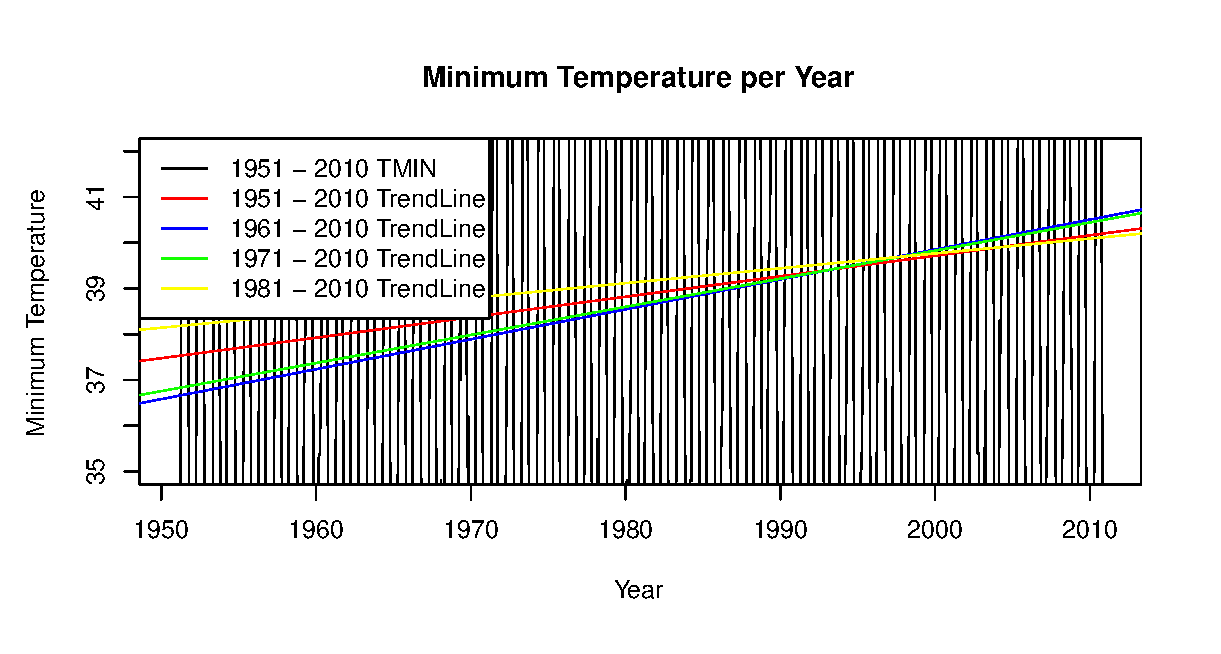
\includegraphics{Figures/Prob9}

\begin{Shaded}
\begin{Highlighting}[]
\NormalTok{printPartC <-}\StringTok{ }\KeywordTok{c}\NormalTok{(}\KeywordTok{paste}\NormalTok{(}\StringTok{'Slope for 1951-2010 TrendLine:'}\NormalTok{,slope[}\DecValTok{1}\NormalTok{]), }
                \KeywordTok{paste}\NormalTok{(}\StringTok{'Slope for 1961-2010 TrendLine:'}\NormalTok{,slope[}\DecValTok{2}\NormalTok{]), }
                \KeywordTok{paste}\NormalTok{(}\StringTok{'Slope for 1971-2010 TrendLine:'}\NormalTok{,slope[}\DecValTok{3}\NormalTok{]), }
                \KeywordTok{paste}\NormalTok{(}\StringTok{'Slope for 1981-2010 TrendLine:'}\NormalTok{,slope[}\DecValTok{4}\NormalTok{]))}
\KeywordTok{matrix}\NormalTok{(printPartC)}
\end{Highlighting}
\end{Shaded}

\begin{verbatim}
##      [,1]                                               
## [1,] "Slope for 1951-2010 TrendLine: 0.0447627020885443"
## [2,] "Slope for 1961-2010 TrendLine: 0.0654045150125415"
## [3,] "Slope for 1971-2010 TrendLine: 0.0614426494906739"
## [4,] "Slope for 1981-2010 TrendLine: 0.0324715468483712"
\end{verbatim}
\newpage
\begin{Shaded}
\begin{Highlighting}[]
\CommentTok{#Problem 10, Exercise 2.9}

\KeywordTok{setwd}\NormalTok{(}\StringTok{'C:/Users/Stephen Giang/Documents/Math336Files/data'}\NormalTok{)}
\NormalTok{readData <-}\StringTok{ }\KeywordTok{read.csv}\NormalTok{(}\StringTok{'NOAAGlobalT.csv'}\NormalTok{)}

\NormalTok{t <-}\StringTok{ }\KeywordTok{seq}\NormalTok{(}\DecValTok{1880}\NormalTok{,}\DecValTok{2017}\NormalTok{, }\DataTypeTok{by=}\NormalTok{(}\DecValTok{1}\OperatorTok{/}\DecValTok{12}\NormalTok{))}
\NormalTok{y1 <-}\StringTok{ }\NormalTok{readData[}\DecValTok{1800}\NormalTok{,}\DecValTok{4}\OperatorTok{:}\KeywordTok{dim}\NormalTok{(readData)[}\DecValTok{2}\NormalTok{]]}
\NormalTok{y2 <-}\StringTok{ }\NormalTok{readData[}\DecValTok{1810}\NormalTok{,}\DecValTok{4}\OperatorTok{:}\KeywordTok{dim}\NormalTok{(readData)[}\DecValTok{2}\NormalTok{]]}

\KeywordTok{plot}\NormalTok{(t, y1, }\StringTok{'l'}\NormalTok{,}\DataTypeTok{col=}\StringTok{'red'}\NormalTok{,}\DataTypeTok{ylab =} \StringTok{'Temperature'}\NormalTok{, }\DataTypeTok{xlab =} \StringTok{'Year'}\NormalTok{ ,}
     \DataTypeTok{main =} \StringTok{'Temperature Anomaly Time Series'}\NormalTok{)}
\KeywordTok{lines}\NormalTok{(t, y2, }\StringTok{'l'}\NormalTok{,}\DataTypeTok{col=}\StringTok{'blue'}\NormalTok{)}

\NormalTok{text <-}\StringTok{ }\KeywordTok{c}\NormalTok{(}\StringTok{'Lat: 32.5, Lon: 357.5'}\NormalTok{, }\StringTok{'Lat: 37.5, Lon: 47.5'}\NormalTok{)}
\KeywordTok{legend}\NormalTok{(}\StringTok{'topleft'}\NormalTok{, }\DataTypeTok{legend =}\NormalTok{ text, }\DataTypeTok{col =} \KeywordTok{c}\NormalTok{(}\StringTok{'red'}\NormalTok{,}\StringTok{'blue'}\NormalTok{), }\DataTypeTok{lty=}\DecValTok{1}\NormalTok{, }\DataTypeTok{cex=}\DecValTok{1}\NormalTok{)}
\end{Highlighting}
\end{Shaded}

\includegraphics{Assignment1_files/figure-latex/prob10-1.pdf}

\end{document}
